Para el circuito de la figura \ref{4.0}, se desea calcular la frecuencia de oscilación y verifica si se cumple la condición de amplitud:

\begin{figure}[h]
\centering
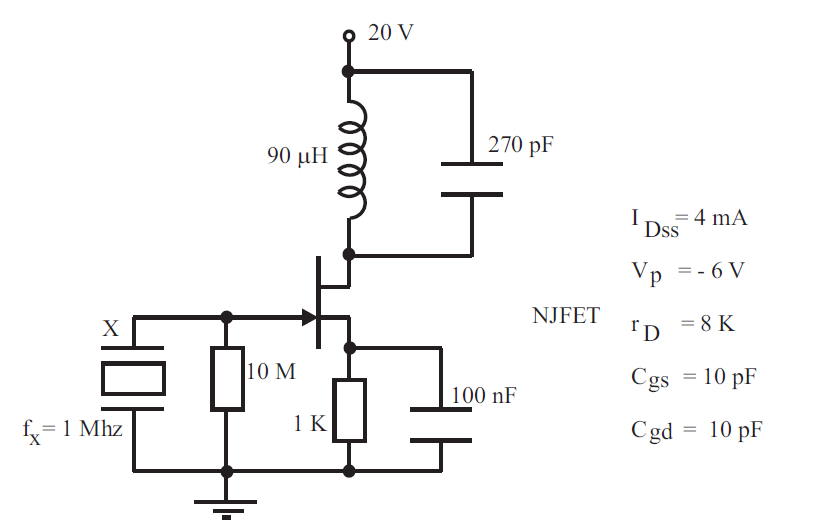
\includegraphics[width=0.5\linewidth]{images/circuito_3.png}
\caption{Oscilador con cristal.}
\label{4.0}
\end{figure}

En equivalente de alterna es, sabiendo que el capacitor de $100 n F$ actúa como un corto circuito, y conociendo el modelo del alterna del $JFET$:



\begin{figure}[H]
  	\centering
		 \begin{circuitikz}[scale=1.5][american]
		 \draw
	     (0,0) 	node[njfet](fet1){JFET}
	      ;
	      % Conectores
         \draw
	     (fet1.G) -- ++(-0.3,0) node[circ] node[above]{$V_G'$} -- ++(-1,0) -- ++(0,-2) -- ++(8.5,0) -- ++(0,1.27) -- ++(0,2.18)--(6,1.27) node[above]{$V_G$} -- (5.2,1.27) 
	     {}
	     ;
	     \draw
	     (fet1.G) -- ++(-0.3,0) to [R, l_=$10M\Omega$] ++(0,-1.2) node[ground]
	     {};
	     
	     \draw
	     (fet1.S) -- ++(0,-0.2) node [ground]
	     {};
	     \draw 
	     (fet1.D) -- (0,1.27) -- ++(1,0) node[circ] to [R,l^=$r_D$]  ++(0,-2.05) node [ground]{};
	     
	     \draw 
	     (1,1.27) -- (1.8,1.27) to [L,l=$L$] ++(0,-2.05) node[ground]
	     {};
	     \draw 
	     (1.8,1.27) node[circ]-- (2.5,1.27) to [C,l=$270 pF$] ++(0,-2.05) node[ground]
	     {};
	     
	     \draw
	     (2.5,1.27) node[circ] to [C,l_=$C_{gs}$] (4,1.27) node[circ] 
 	     {};
 	     
 	     \draw
	     (4,1.27) to [C,l=$C_{gd}$] ++(0,-2.05) node[ground]
 	     {};
 	     
 	     \draw
 	     (4,1.27)--(5.2,1.27) node[circ] to [PZ, l=$XTAL$] ++(0,-2.05) node[ground]
 	     {};
 	     

	    
		\end{circuitikz}
    \caption[Equivalente de alterna]{Equivalente de alterna.}
    \label{4.1}
\end{figure}

Recortando el lazo entre los nodos $V_G$ y $V_G'$, obtenemos así el circuito a lazo abierto como se observa en la figura \ref{4.2}. En ella no se puede saber a priori cuáles son las reactancias $X_1$, $X_2$ y $X_3$ que determinan la condición de fase en este tipo de redes LC. Es por eso que se adoptan las reactancias en paralelo como se indican en las expresiones \ref{eq:4.0}, \ref{eq:4.1}, \ref{eq:4.2}, a la frecuencia del cristal oscilador $f_o = 1 MHz$.

\begin{figure}[H]
  	\centering
		 \begin{circuitikz}[scale=1.5][american]
		 \draw
	     (0,0) 	node[njfet](fet1){JFET}
	      ;
	      % Conectores
         \draw
	     (fet1.G) -- ++(-0.3,0) node[ocirc] node[above]{$V_G'$}
	     {}
	     ;
	     \draw
	     (5.2,1.27) -- (6.6,1.27) to [R, l=$10M\Omega$] ++(0,-2.05) node[ground]
	     {};
	     \draw
	     (6.6,1.27) node[circ] -- (7,1.27) node[ocirc] node [above]{$V_G$}
	     {};
	     
	     
	     \draw
	     (fet1.S) -- ++(0,-0.2) node [ground]
	     {};
	     \draw 
	     (fet1.D) -- (0,1.27) -- ++(1,0) node[circ] to [R,l^=$r_D$]  ++(0,-2.05) node [ground]{};
	     
	     \draw 
	     (1,1.27) -- (1.8,1.27) to [L,l=$L$] ++(0,-2.05) node[ground]
	     {};
	     \draw 
	     (1.8,1.27) node[circ]-- (2.5,1.27) to [C,l=$270 pF$] ++(0,-2.05) node[ground]
	     {};
	     
	     \draw
	     (2.5,1.27) node[circ] to [C,l_=$C_{gs}$] (4,1.27) node[circ] 
 	     {};
 	     
 	     \draw
	     (4,1.27) to [C,l=$C_{gd}$] ++(0,-2.05) node[ground]
 	     {};
 	     
 	     \draw
 	     (4,1.27)--(5.2,1.27) node[circ] to [PZ, l=$XTAL$] ++(0,-2.05) node[ground]
 	     {};
 	     
 	     
 	     
	    % \draw
	     %(1,1.27) to [L,l_=$L$] (3,1.27) node[circ] to [C,l_=$C2$] %(3,-0.78) -- (0,-0.78){} ;
	     
	     %\draw 
	     %(1,1.27) -- (1,2.2) to [R, l_=$R_L$] (3,2.2) -- (3,1.27) to %++(0.4,0)node[above]{$V_t$}{};
	    
		\end{circuitikz}
    \caption[Equivalente de alterna]{Equivalente de alterna a lazo abierto.}
    \label{4.2}
\end{figure}


\begin{equation}
\label{eq:4.0}
X_1(f_o) = jX_L \parallel jX_{270pF} \approxeq j 13.9 K \Omega 
\end{equation}


\begin{equation}
\label{eq:4.1}
X_3(f_o) = jX_{C_{gs}} \approxeq -j 15.9 K \Omega
\end{equation}


\begin{equation}
\label{eq:4.2}
X_2(f_o) = jX_{C_{gd}} \parallel Z_{XTAL}
\end{equation}

La condición de fase es: 

\begin{equation}
\label{eq:4.3}
X_1(f_o)+X_2(f_o)+X_3(f_o) = 0
\end{equation}

Despejando $X_2(f_o)$ se obtiene $X_2(f_o)\approxeq 2K \Omega$. Luego, se aplica un equivalente de thevenin desde $X_1$:

\begin{equation}
\label{eq:4.4}
Z_{eq} = jX_3(f_o) + jX_2(f_o) \parallel 10M\Omega \approxeq 800 \Omega -j15.5 K\Omega 
\end{equation}

En términos de admitancia:

\begin{equation}
\label{eq:4.5}
Y_{eq} = \frac{1}{Z_{eq}} \approxeq 3.3 \micro \mho +j64.3 \micro \mho \equiv \frac{1}{R_{eq}} + j2\pi f_o \cdot C_{eq} 
\end{equation}

Se obtiene entonces, en paralelo, una impedancia equivalente que consta de una resistencia $R_{q}\approxeq300 K\Omega$ en paralelo con un capacitor $C_{eq} \approxeq10.23 pf$. EL circuito entonces posee la forma de la figura \ref{4.3}.  

\begin{figure}[H]
  	\centering
		 \begin{circuitikz}[scale=1.5][american]
		 \draw
	     (0,0) 	node[njfet](fet1){JFET}
	      ;
	      % Conectores
         \draw
	     (fet1.G) -- ++(-0.3,0) node[ocirc] node[above]{$V_G'$}
	     {}
	     ;
	     \draw
	     (fet1.S) -- ++(0,-0.2) node [ground]
	     {};
	     \draw 
	     (fet1.D) -- (0,1.27) -- ++(1,0) node[circ] to [R,l^=$r_D$]  ++(0,-2.05) node [ground]{};
	     
	     \draw 
	     (1,1.27) -- (1.8,1.27) to [L,l=$L$] ++(0,-2.05) node[ground]
	     {};
	     \draw 
	     (1.8,1.27) node[circ]-- (2.5,1.27) to [C,l=$270 pF$] ++(0,-2.05) node[ground]
	     {};
	     
	     \draw
	     (2.5,1.27) node[circ] -- (4,1.27) node[circ] 
 	     {};
 	     
 	     \draw
	     (4,1.27) to [C,l=$C_{eq}$] ++(0,-2.05) node[ground]
 	     {};
 	     
 	     \draw
 	     (4,1.27)--(5.2,1.27) node[circ] to [R, l=$R_{eq}$] ++(0,-2.05) node[ground]
 	     {};

		\end{circuitikz}
    \caption[Equivalente de alterna]{Equivalente de thevenin.}
    \label{4.3}
\end{figure}

\newpage
Por lo que la frecuencia de oscilación es: 

\begin{equation}
\label{eq:4.6}
f_o = \frac{1}{2\pi} \cdot \sqrt{\frac{C_{eq} + 270 pF}{L\cdot C_{eq} \cdot 270pF}} \approxeq 1.002 MHz
\end{equation}

Claramente el resultado anterior es el esperado por lo que los efectos de carga y/o desviaciones de los elementos no lograrían desviar de manera significativa a la frecuencia de oscilación deseada. 

Ahora bien, se sabe que la condición de amplitud es: 

\begin{equation}
\label{eq:4.7}
g_m \cdot R_{eq}\parallel r_D \geq \frac{X_1}{X_2} \approxeq 7
\end{equation}

Por lo que se tiene que analizar la polarización del JFET para asegurar la condición anterior tal que  la tras-conductancia del dispositivo sea $g_m \geq 0.899 \mu \mho$. Para ello se recurre a un análisis de polarización en el cual la corriente de Drain $I_D$ depende de la polarización en inversa $V_{gs}$:

\begin{equation}
\label{eq:4.8}
I_D = I_{DSS}\cdot (1-\frac{V_{gs}}{V_p})^2
\end{equation}

Pero dado que la polarización depende de la resistencia en el Source $1K\Omega$ (ya que en continua el capacitor en paralelo actúa como un circuito abierto): 

\begin{equation}
\label{eq:4.9}
I_D = - \frac{V_{gs}}{1K\Omega}
\end{equation}

Por lo que la intersección entre las curvas dadas por las ecuaciones \ref{eq:4.8} y \ref{eq:4.9} sería el punto de operación $(I_{DQ};V_{gsQ})$. En la figura \ref{4.6} se grafican dichas curvas por lo que se obtiene $I_{DQ}\approxeq1.88mA$ y $V_{gsQ}\approxeq-1.88V$. La tras-conductancia $g_m$ está dada por la siguiente expresión:

\begin{equation}
\label{eq:4.91}
g_m= -2\frac{I_{DSS}}{V_p}\cdot (1-\frac{V_{gsQ}}{V_p}) \approxeq 0.9155 \mu \mho
\end{equation}

Dado que es mayor al valor límite que cumple la condición de arranque y amplitud, podemos asegurar que el circuito efectivamente va a oscilar.


\begin{figure}[h]
\centering
\fbox{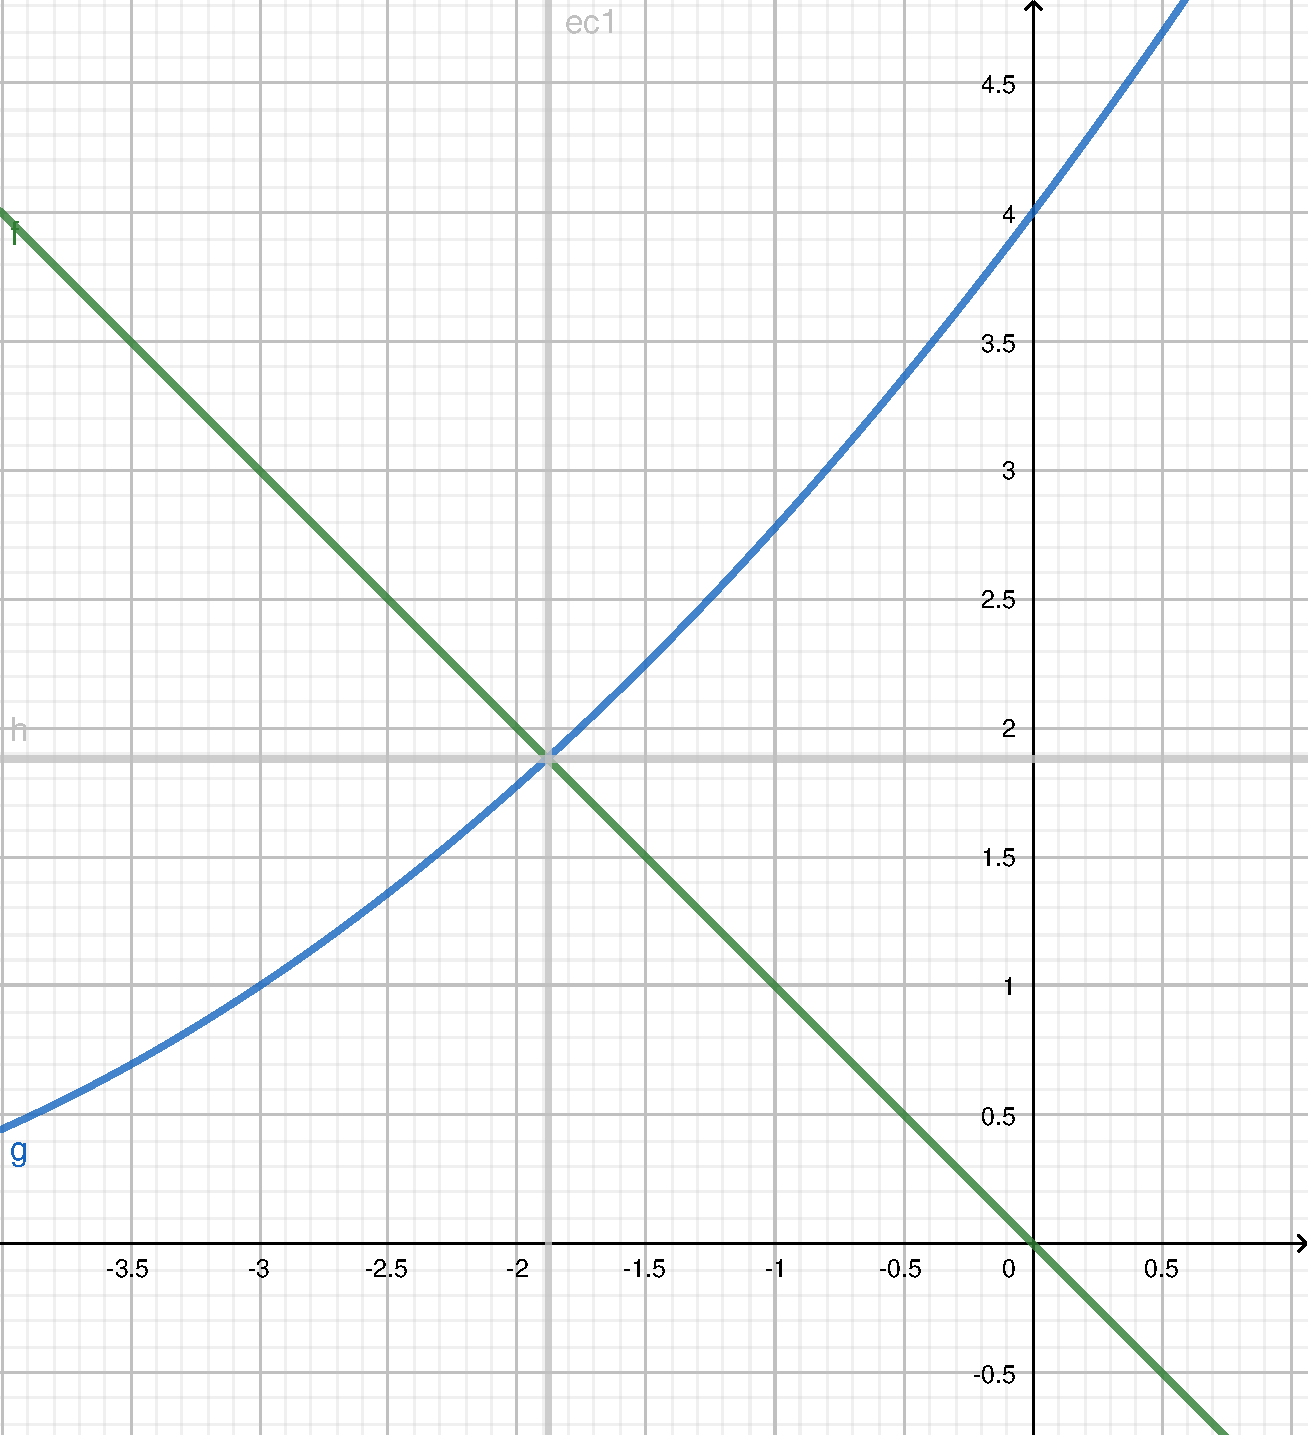
\includegraphics[width=0.7\linewidth]{images/geogebra.pdf}}
\caption{Intersección entre curvas. Eje horizonal medido en $V$. Eje vertical medido en $mA$}
\label{4.6}
\end{figure}




